\documentclass{article}
\usepackage{tikz}

\begin{document}

\begin{figure}[h]
    \centering
    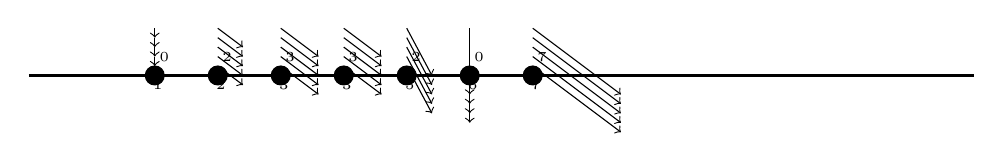
\begin{tikzpicture}[scale=0.8]
        % Draw the road
        \draw[thick] (-1,0) -- (14,0);
        
        % Draw the cars and their preferences
        \foreach \x/\p/\t in {1/0/1, 2/2/2, 3/3/3, 4/3/3, 5/2/5, 6/0/6, 7/7/7} {
            \filldraw[black] (\x,0) circle (0.15);
            \foreach \y in {0.15,0.3,...,0.9} {
                \draw[->] (\x,\y) -- ++(\p*0.2,-\t*0.15);
            }
            \node at (\x+0.15,0.3) {\tiny \p};
            \node at (\x+0.05,-0.15) {\tiny \t};
            \draw[ultra thick] (\x-0.15,0) -- (\x+0.15,0);
        }
    \end{tikzpicture}
    
    \caption{Parking outcome under the preference list $(7,5,3,3,2)$. The number on the car is its original place in line and the number in the thought bubble above the car is that car's preferred parking spot.}
    \label{fig:parking_outcome}
\end{figure}

\end{document}